\subsection{Ablenkung im magnetischen Feld}
In diesem Abschnitt werden die Messungen zur Ablenkung im magnetischen Feld ausgewertet.

Das Helmholtzspulenpaar, welches zur Erzeugung des Magnetfeldes verwendet wird,
ist charakterisiert durch die Windungszahl $N = 20$
und den Radius $R = \SI{0.282}{\meter}$.
% L = ?
%TODO: verif.

\subsubsection{spezifische Ladung der Elektronen}
\label{sec:auswertung:502:spezifische_elektronenladung}

Um die spezifische Ladung der Elektronen zu bestimmen,
wird für jeden Skalenabschnitt der zur Ablenkung des Elektronenstrahls dorthin benötigte Spulenstrom $I$ notiert,
wie in \autoref{sec:durchfuehrung:502} beschrieben.
Diese Messwerte für verschiedene Beschleunigungsspannungen $U_\text{B}$ sind in \autoref{tab:mess_502} aufgeführt.

\begin{table}
  \centering
  \caption{Messwerte für den Abstand $D$ und die Stromstärke $I$.}
  \label{tab:mess_502}
  \begin{tabular}{S | S S S S S}
  \toprule
  {$U_\text{B} \mathbin{/} \si{\volt}$} &
  {250} &
  {300} &
  {350} &
  {400} &
  {420} \\
  \midrule
  {$D \mathbin{/} \si{\centi\meter}$} &
  \multicolumn{5}{c}{$I \mathbin{/} \si{\ampere}$} \\
  \midrule
  \expandableinput{build/tab/V502_tab_b.tex}
  \bottomrule
  \end{tabular}
\end{table}

Um aus diesen Werten nun die spezifische Elektronenladung zu bestimmen,
wird zunächst die messbare Größe $\frac{D}{L^2 + D^2}$ berechnet
% wobei die Ablenkung $D$ auf dem Leuchtschirm offensichtlich  abhängt,
und anschließend anhand von \autoref{eqn:formel_verschiebung} eine Regressionsgerade bestimmt.
Aus der so erhaltenen Steigung
\begin{equation*}
  a \wedgeq \frac{1}{\sqrt{8 U_\text{B}}}
\end{equation*}
kann durch Umstellen der zuvor genannten Gleichung zu
\begin{equation*}
  \frac{e_0}{m_0} = 8 U_\text{B} a^2
\end{equation*}
und Einsetzen der jeweiligen Beschleunigungsspannung $U_\text{B}$
die spezifische Ladung ermittelt werden.
Die Steigungen der Ausgleichgeraden und daraus bestimmte spezifische Elektronenladungen für verschiedene $U_\text{B}$
sind in \autoref{tab:a_502} aufgeführt;
die Regressionsgeraden sind in \autoref{fig:a_502} visualisiert.

\begin{table}[H]
  \centering
  \caption{Steigung der Ausgleichgeraden und daraus bestimmte spezifische Elektronenladungen.}
  \label{tab:a_502}
  \begin{tabular}{S S S}
  \toprule
  {$U_\text{B} \mathbin{/} \si{\volt}$} &
  {$a \mathbin{/} \si{\per\meter\per\tesla}$} &
  {$\frac{e_0}{m_0} \mathbin{/} \SI{e11}{\coulomb\per\kilo\gram}$} \\
  \midrule
  250 & 8823.8(1194) & 1.56(4) \\
  300 & 8152.6(1460) & 1.60(6) \\
  350 & 7568.7(1146) & 1.60(5) \\
  400 & 7216.7(1224) & 1.67(6) \\
  420 & 6987.4(1240) & 1.64(6) \\
  \bottomrule
  \end{tabular}
\end{table}

Im Mittel ergibt sich $\frac{e_0}{m_0} = \SI{1.613(24) e11}{\coulomb\per\kilo\gram}$.

\begin{figure}
   \centering
    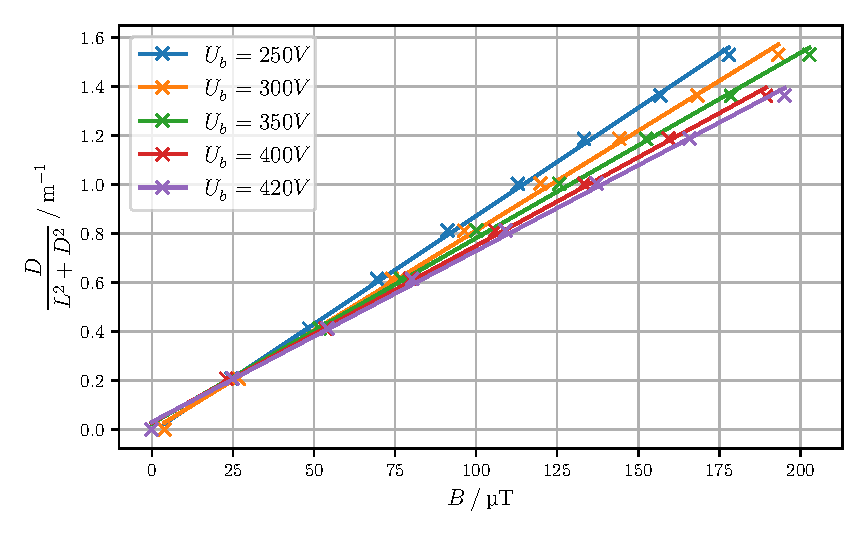
\includegraphics[width=\textwidth]{build/plt/V502_1.pdf}
    \caption{Transformierte Messwerte und Regressionsgeraden in Abhängigkeit des Magnetfeldes.}
    \label{fig:a_502}
\end{figure}


% \clearpage
\FloatBarrier
\subsubsection{Bestimmung des lokalen Erdmagnetfelds}
\label{sec:auswertung:502:erdmagnetfeld}

Gemäß dem in \autoref{sec:durchfuehrung:502:erdmagnetfeld} beschriebenen Verfahren
wird für drei verschiedene Beschleunigungsspannungen
der Spulenstrom $I_\text{hor}$ ermittelt,
der benötigt wird,
um die Horizontalkomponente des Erdmagnetfelds auszugleichen.
Die Messwerte zeigt \autoref{tab:erdmagnetfeld}.

\begin{table}
  \centering
  \caption{Ausgleichender Spulenstrom für verschiedene Beschleunigungsspannungen.}
  \label{tab:erdmagnetfeld}
  \begin{tabular}{S S}
  \toprule
  {$U_\text{B} \mathbin{/} \si{\volt}$} &
  {$I_\text{hor} \mathbin{/} \si{\ampere}$} \\
  \midrule
  150 & 0.49 \\
  160 & 0.46 \\
  170 & 0.45 \\
  \bottomrule
  \end{tabular}
\end{table}

Der Mittelwert aus den drei Messungen des Stroms beträgt $\bar{I}_\text{hor} = \SI{0.467(12)}{\ampere}$.
Daraus ergibt sich nach \autoref{eqn:magn_flussdichte} eine magnetische Flussdichte von
$B_\text{hor} = \SI{29.8(8)}{\micro\tesla}$.
Unter Berücksichtigung des mittels Inklinatorium bestimmten Inklinationswinkels
von $\varphi = \SI{54}{\degree}$
ergibt sich für die Totalintensität des Erdmagnetfelds
\[ B_\text{total} = \frac{B_\text{hor}}{\sin{\varphi}} = \SI{36.79(95)}{\micro\tesla} \ . \]
